\subsection{Trilinear Interpolation} \label{add:trilinear_interpolation}

    \begin{wrapfigure}{r}{0.41\textwidth}
        \centering
        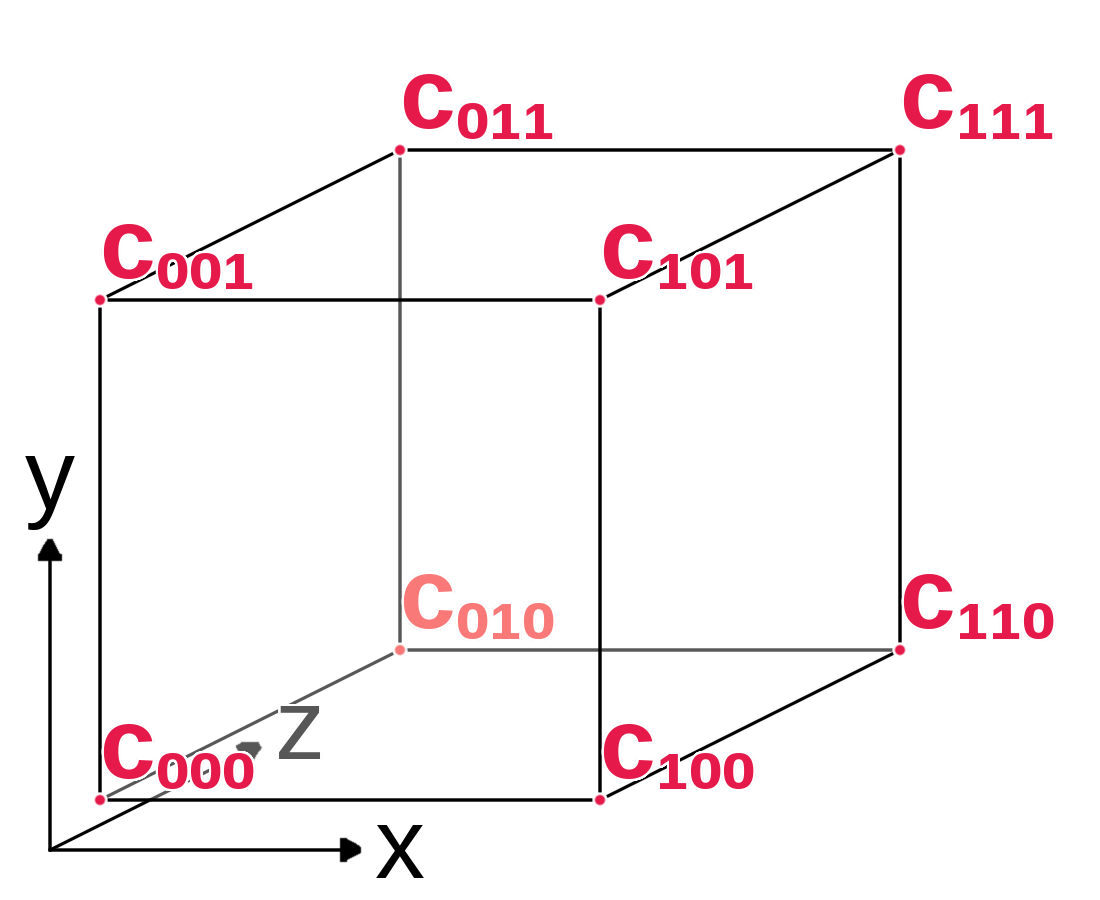
\includegraphics[width=1\textwidth]{bfield/trilinear_interpolation}
        \caption{\label{fig:trilinear_interpolation} Trilinear interpolation visual interpretation.}
    \end{wrapfigure}

Trilinear Interpolation~\cite{bourke1999interpolation} is a method that can be used to compute the value in a tridimensional space given that a regular grid of $(x,y,z)$ points and the value of the function to be interpolated $f$ is known for this set of points.

Given a point $(x,y,z)$ from which the value $f(x,y,z)$ is to be estimated, it is easy to see that the value lies inside a cube in the given regular grid with borders $(x_0, x_1)$, $(y_0, y_1)$, $(z_0, z_1)$, so that the values $c_{000}$, $c_{001}$, $c_{010}$, $c_{011}$, $c_{100}$, $c_{101}$, $c_{110}$, $c_{111}$, defined as $c_{000} = f(x_0, y_0, z_0)$, $c_{001} = f(x_0, y_0, z_1)$ and so on are already known, as seen in Figure \ref{fig:trilinear_interpolation}.

From this data, the values $x_d$, $y_d$ and $z_d$ can be obtained as:
    \begin{equation*}
        x_d = \frac{x - x_0}{x_1 - x_0},~ y_d = \frac{y - y_0}{y_1 - y_0},~ z_d = \frac{z - z_0}{z_1 - z_0}\,,
    \end{equation*}
from which linear interpolation can be done ``in steps'', first for $x$:
    \begin{align*}
        c_{00} = c_{000}(1 - x_d) + c_{100}x_d\\
        c_{01} = c_{001}(1 - x_d) + c_{101}x_d\\
        c_{00} = c_{010}(1 - x_d) + c_{110}x_d\\
        c_{00} = c_{011}(1 - x_d) + c_{111}x_d\,,
    \end{align*}
then for $y$:
    \begin{align*}
        c_0 = c_{00}(1 - y_d) + c_{10}y_d\\
        c_1 = c_{01}(1 - y_d) + c_{11}y_d\\\,,
    \end{align*}
and finally for $z$:
    \begin{equation*}
        c = c_0(1 - z_d) + c_1z_d\,,
    \end{equation*}
with $c$ denoting the interpolated $\tilde{f}(x,y,z)$ value.